\documentclass[conference]{IEEEtran}

\usepackage{graphicx}
\usepackage{amsmath, amssymb}
\usepackage{hyperref}
\usepackage{caption}
\usepackage{cite}
\usepackage{float}

\title{D.I.A.G.R.A.M.: Development of Image Analysis for Graph Recognition And Modeling}

\author{
    \IEEEauthorblockN{Filippo Garagnani, Saverio Napolitano, Nicola Ricciardi}
    \IEEEauthorblockA{
        'Computer Vision and Cognitive System' course \\
        \textit{Università di Modena e Reggio Emilia}
    }
}

\begin{document}

\maketitle

\begin{abstract}
This report describes D.I.A.G.R.A.M., a system for diagram recognition and generation. We present its architecture, the logic behind deterministic algorithms and the training of its deep learning components. The project aims to transform visual diagram input into structured representations.
\end{abstract}

\section{Introduction}
Diagrams are crucial in education, documentation, and many other fields. Developing a system that automatically understands and generates diagrams may reveal helpful for having high-quality, easily editable representations. This, however, poses challenges involving classification, shape detection, structure interpretation and symbolic representation. Our project proposes a modular architecture to tackle these tasks.

% System Architecture
\section{System Architecture}
Figure~\ref{fig:pipeline} illustrates the full pipeline, composed of four main modules: the Classifier, Extractor, Transducer, and Compiler. Each module is designed to process and transform the handwritten diagram image progressively toward a structured output.

\begin{figure}[H]
\centering
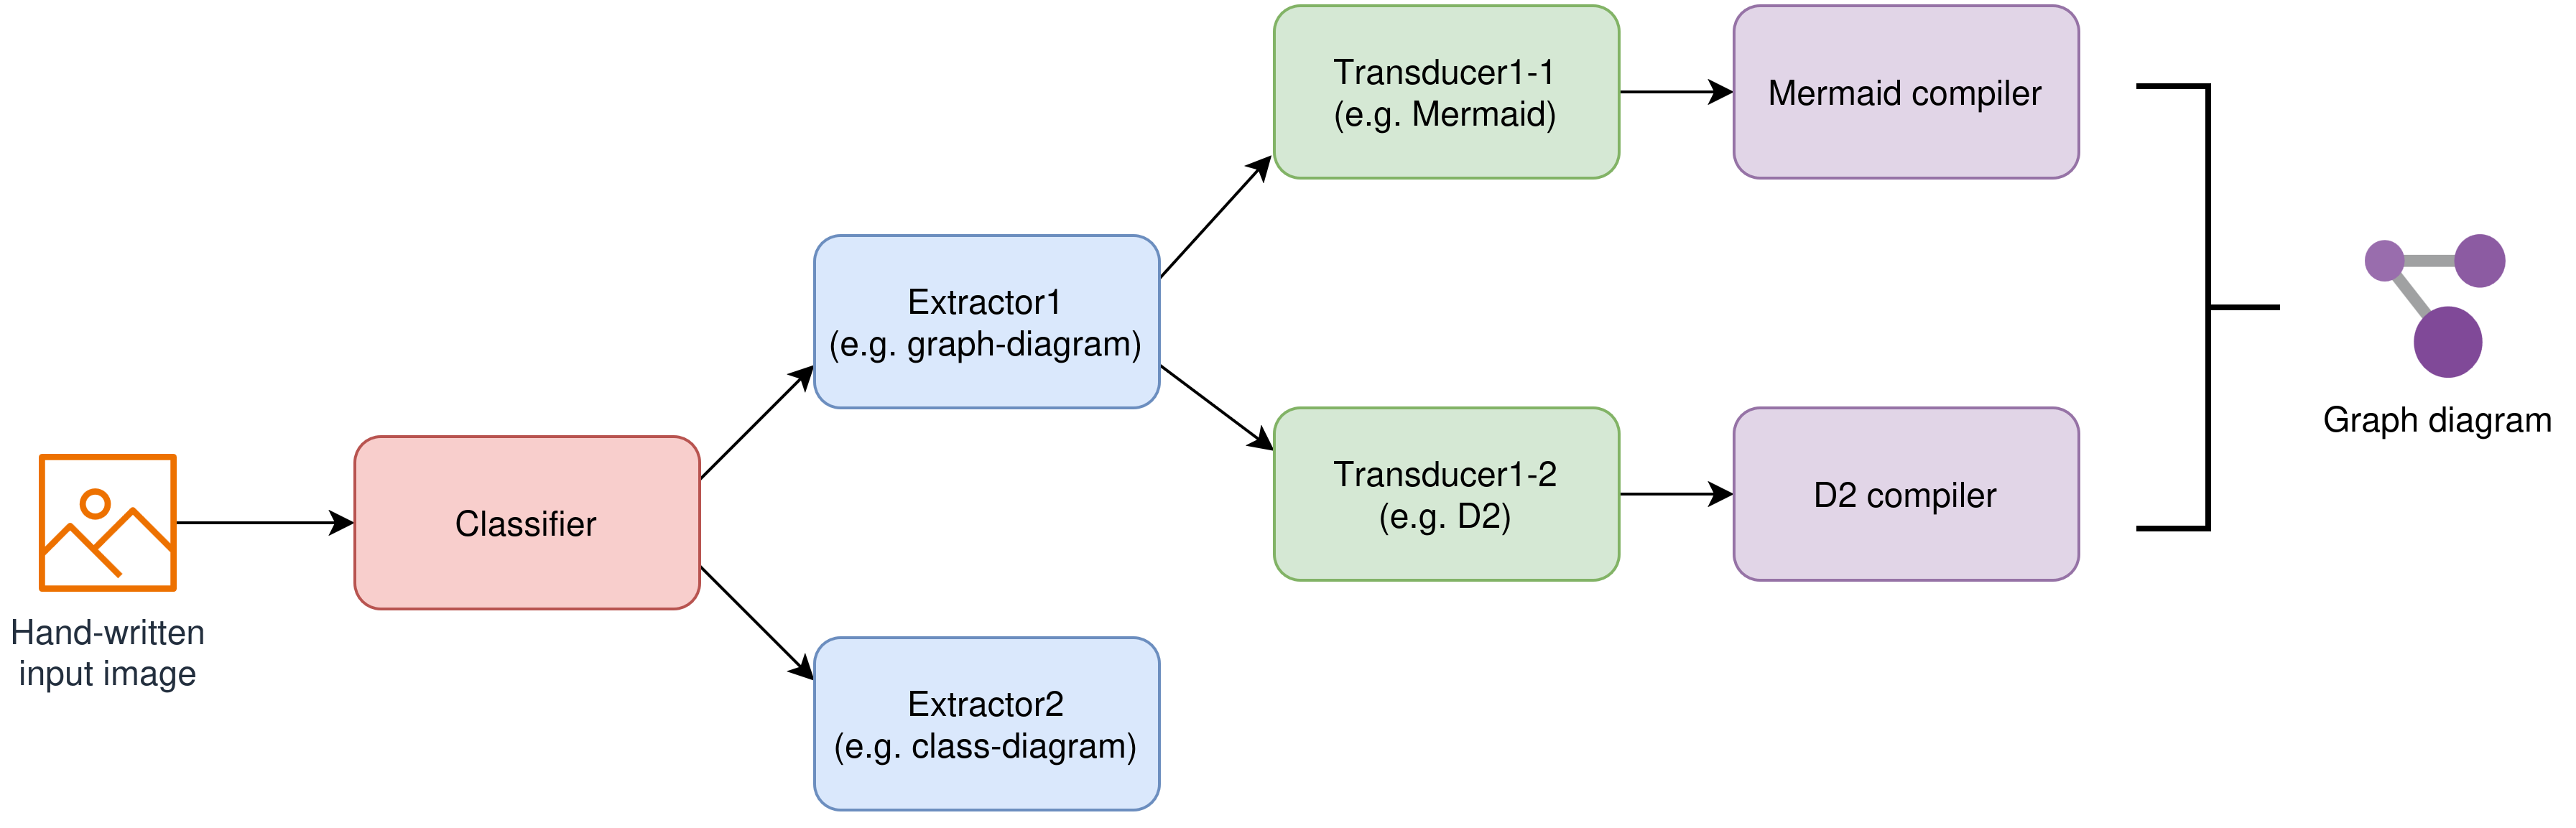
\includegraphics[width=\linewidth]{overview.png}
\caption{Overview of the D.I.A.G.R.A.M. system architecture.}
\label{fig:pipeline}
\end{figure}

The Classifier is able to recognize the category of the hand-written diagram that the user submitted as input. This is necessary in order for the system to know to which Extractor pass the data. This module is able to apply object detection and semantic recognition to represent the diagram in a unified way. After that, the representation is sent to the Transducer, which converts the data in a Markup language of choice. The Markup language content is therefore sent to the Compiler, thus generating the high-quality and editable diagram in .png format.

\subsection{Classifier Module}
The Classifier is the first component of the pipeline. It is able to tell to which category a given image of an handwritten diagram belongs to. This is necessary in order to later know the Extractors that can process the input image.
\subsection{Extractor Module}
The Extractor is the key component of the D.I.A.G.R.A.M. system, able to transform the raw diagram image into a structured, category-agnostic representation.
The Extractor recognizes the diagram's components, such as shapes, lines, and text, through an object detection network, and organizes them into a unified format. This representation serves as the foundation for the subsequent Transducer module, which converts the structured data into a domain-specific markup language.
\subsection{Transducer Module}
The Transducer is responsible for converting the unified, agnostic representation of a diagram into a domain-specific markup language. 
This transformation enables the subsequent Compiler module to generate high-quality visual outputs.
\subsection{Compiler Module}
The Compiler module is the final stage of the D.I.A.G.R.A.M. pipeline. 
Its primary role is to take the structured representation of the diagram, expressed in a markup language (e.g., Mermaid.js), and generate a high-quality diagram in a visual format such as PNG. 

% 
% Flowchart Diagram
%
\section{Flowchart Diagram Recognition}

\subsection{Internal Representation}
In order to pass data through the components of the pipeline in a unified way, it was necessary to decide upon an internal representation of the flowchart diagram. It consists of \textbf{elements} and \textbf{relations}. The latter are linked to at least one element. Every element has a \textit{category} and possibly some \textit{inner} and \textit{outer text}. Every relation has a \textit{category} too, either a \textit{source} or \textit{target element} or both, and possibly \textit{text} related to it.

This internal representation is generated from the image provided by the user by the Extractor module, while it is parsed and converted to a markup language of choice by the Transducer. 

\subsection{Classifier Module}
\subsubsection{Preprocessing}
TODO \\

\subsubsection{Model}
TODO \\

\subsection{Extractor Module}
\subsubsection{Preprocessing}
TODO\\
\subsubsection{Bounding Box Detection}
TODO\\
\subsubsection{Content Recognition}
After having determined all the bounding boxes of the diagram image, in order to correctly create the diagram internal representation, there's the need to link together text, elements and relations.\\

\subsubsection{Arrow Orientation}
To later correctly assign arrows to their source and target elements, the need to determine where the tip of an arrow lies. This task involves a few problems, among which determining exactly the arrow shape and its end - because sometimes other pen signs may be found in the bounding box of the arrow itself. [TODO: Dire l'approccio finale usato]. \\

\subsubsection{Text Digitization}
Since the task of converting an image of text into the relative string has already been solved in various ways, we settled upon the Microsoft \textit{Trocr Handwritten} Transformer model; more precisely, the \textit{base} version of it. Every bounding box containing text that has been found is later passed to the model, and the resulting string generated by the model is linked to it.\\

\subsubsection{Text Association}
It can be assumed that every piece of text is linked to one and only one element or relation. So, every bounding box containing text is linked to the nearest element - it being either a relation or an element. The associations that require too long a distance are eliminated further in the algorithm, and the relevant text is discarded.\\

\subsubsection{Element-Text Association}
After that a text box has been assigned to an element, there's the need to understand if the text is either inside or outside the element and whether the text is actually referring to the given element or not. In order to do this, the overlap between the two bounding boxes is computed; if the overlap is over a certain threshold, heuristically decided, the association is kept. Otherwise, the distance between the two bounding boxes is computed - as the distance between their central point. If the distance is over a certain threshold, the association is kept; otherwise, it's discarded.\\

\subsubsection{Relation-Text Association}
After a text box is assigned to a relation, some computation is needed to fully understand how the text is associated to the relation itself. [TODO: Come trova source e target]. The relation bounding box is then split into three different sections. The overlap between the text bounding box and each of the three sections boxes is computed - then, the section with the highest overlap value is then assigned the text under consideration.

\section{Experiments}

\subsection{Classifier}
TODO

\subsection{Object Detection}
TODO

\subsection{Arrow Orientation}
As we've seen in the previous section, the need to find the exact position of an arrow's head arises.
The first algorithmic approach proposed to solve this task - called \textit{Double Clustering} - was as follows: 
\begin{enumerate}
	\item Apply a clustering algorithm to the bounding box.
	\item Suppose that the biggest cluster belongs to the arrow; the other clusters are thought to contain useless elements for this task, and can be discarded.
	\item Find the keypoints of the arrow using SIFT.
	\item Find the two keypoints inside the arrow with maximum distance. Assume that these two points are closely related to the two ends of the arrow.
	\item Run a template matching procedure inside the two clusters to find the head of the arrow.
\end{enumerate}

For Step (1), we tried to employ both Spectral Clustering (see Figure~\ref{fig:spectral_clustering}) and DBSCan (see Figure~\ref{fig:arrow_double_clustering_clusters}).

\begin{figure}[H]
\centering
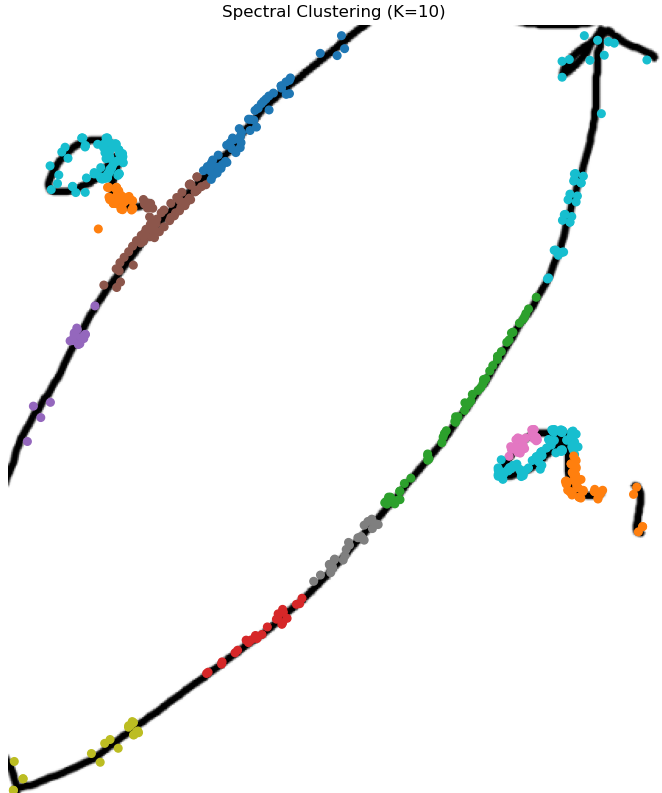
\includegraphics[width=150pt]{spectral_clustering.png}
\caption{The result of Spectral Clustering to one instance of an arrow bounding box in our dataset.}
\label{fig:spectral_clustering}
\end{figure}

\begin{figure}[H]
\centering
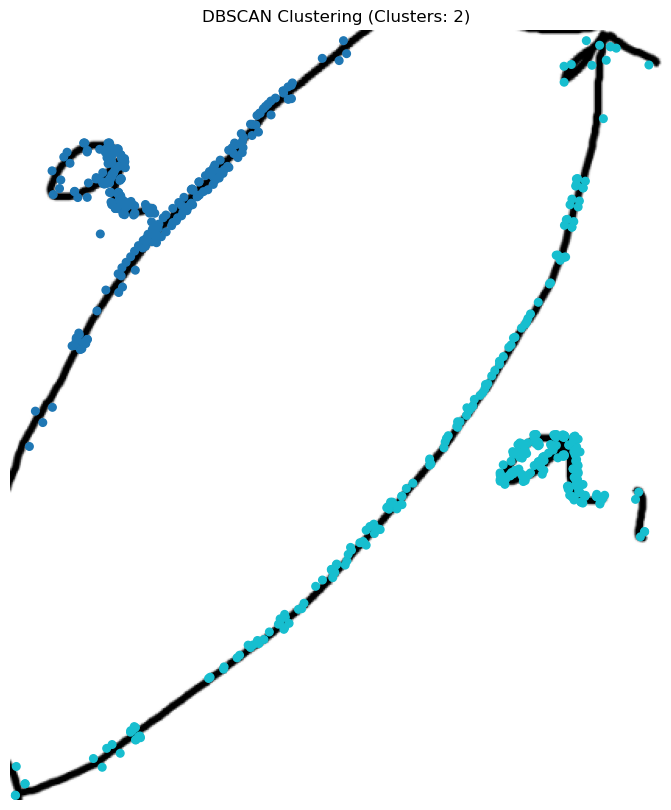
\includegraphics[width=150pt]{arrow_double_clustering_clusters.png}
\caption{The result of DBScan to one instance of an arrow bounding box in our dataset.}
\label{fig:arrow_double_clustering_clusters}
\end{figure}

For Step (3), we used SIFT in order to find keypoints and some descriptors for them - necessary for the later template matching.
During Step (4), we were able to correctly deduce the overall direction of the arrow (see Figure~\ref{fig:arrow_double_clustering_direction}).

\begin{figure}[H]
\centering
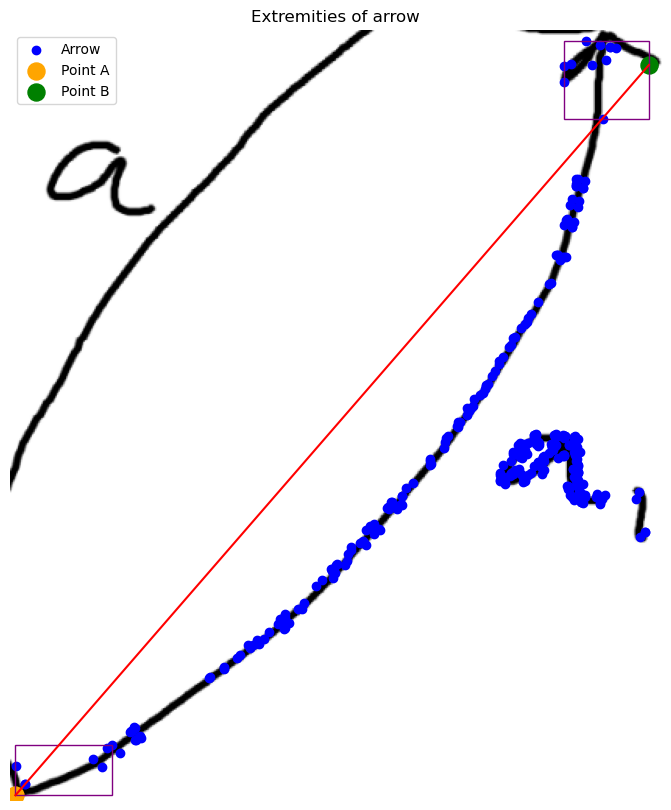
\includegraphics[width=150pt]{arrow_double_clustering_direction.png}
\caption{The estimated direction of the arrow, finding the points that maximize the distance inside the cluster.}
\label{fig:arrow_double_clustering_direction}
\end{figure}

For Step (5), we had previously hand-picked some templates (see Figure~\ref{fig:templates}).

\begin{figure}[H]
\centering
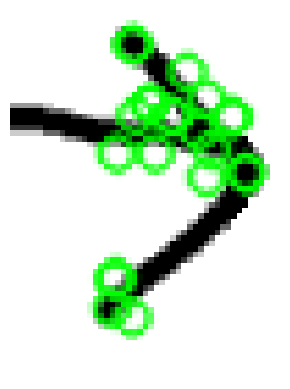
\includegraphics[width=50pt]{templates.png}
\caption{An example of hand-picked template with SIFT descriptors.}
\label{fig:templates}
\end{figure}

However, this approach didn't work as expected (see Figure~\ref{fig:template_matching_fail}). [TODO: Spiegare perchè].

\begin{figure}[H]
\centering
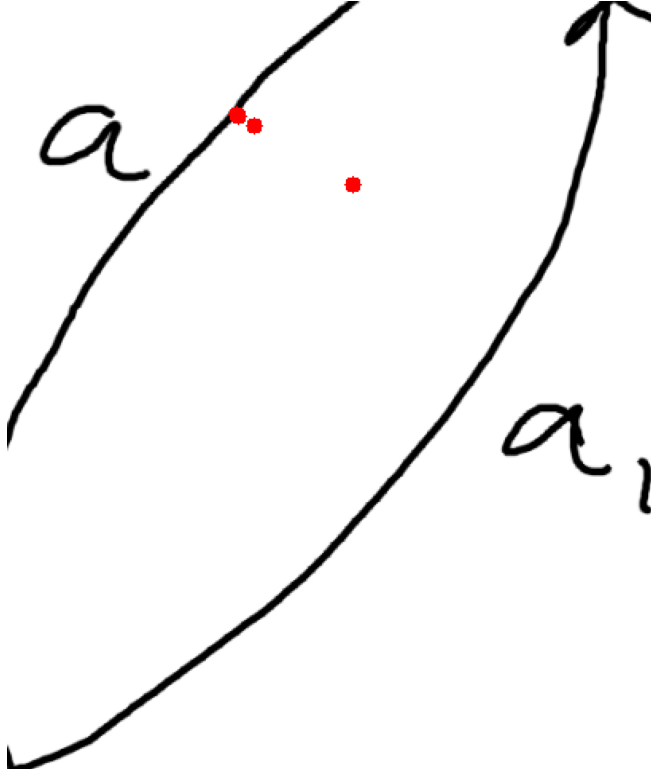
\includegraphics[width=150pt]{template_matching_fail.png}
\caption{The overall result of the algorithm.}
\label{fig:template_matching_fail}
\end{figure}

\subsection{Text Digitization}
In order to choose an appropriate model, some tests were done over our specific dataset employing some different, pre-made models. The average results over the dataset are shown in Table~\ref{tab:text_digitization}.

\begin{table}[htbp]
\caption{Text Distance Metrics}
\centering
\begin{tabular}{lccc}
\hline
\textbf{Model} & \textbf{Hamming} & \textbf{Cosine} & \textbf{Euclidean} \\
\hline
microsoft-trocr-small-printed & 1.392 & 0.150 & 7133 \\
% microsoft-trocr-base-printed & 1.286 & 0.081 & 3594 \\
microsoft-trocr-small-handwritten & \textbf{1.346} & 0.100  & 3947 \\ \hline \textbf{microsoft-trocr-base-handwritten} & 1.549 & \textbf{0.057} & \textbf{3003} \\
\hline
\end{tabular}
\label{tab:text_digitization}
\end{table}

Some examples of the different models applied to our flowchart diagram dataset can be seen in Figure~\ref{fig:text_digitization_results_1} and in Figure~\ref{fig:text_digitization_results_2}.

\begin{figure}[H]
\centering
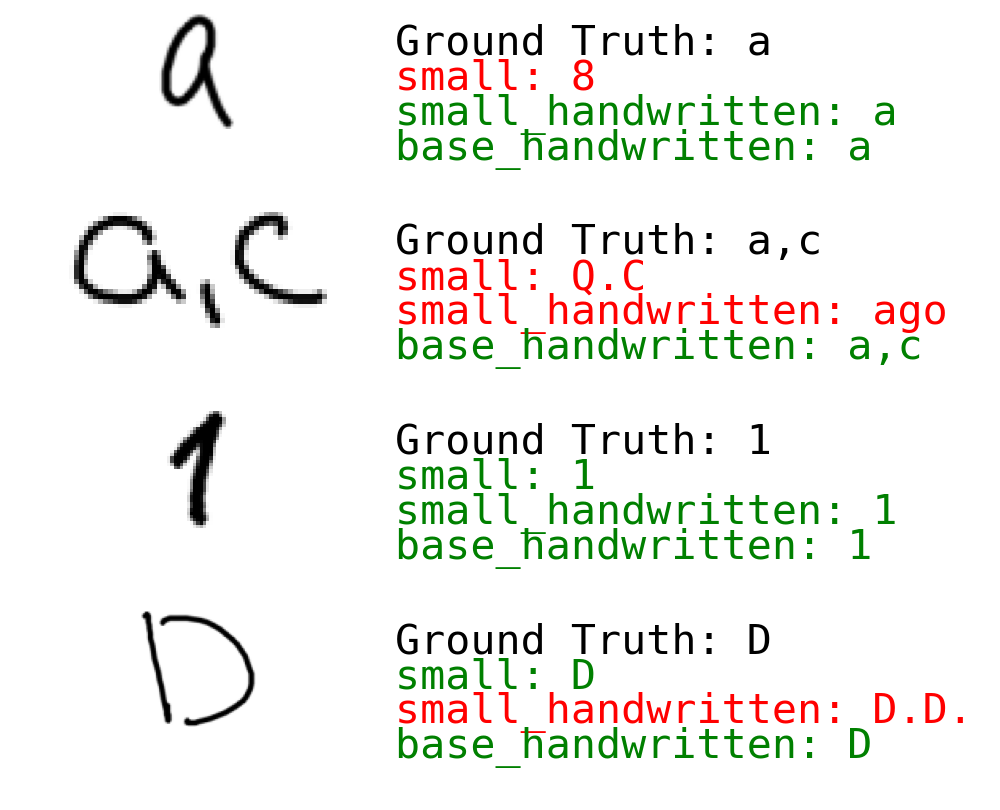
\includegraphics[width=\linewidth]{text_digitization_results_1.png}
\caption{Some random results of the text digitization over the proposed models.}
\label{fig:text_digitization_results_1}
\end{figure}

\begin{figure}[H]
\centering
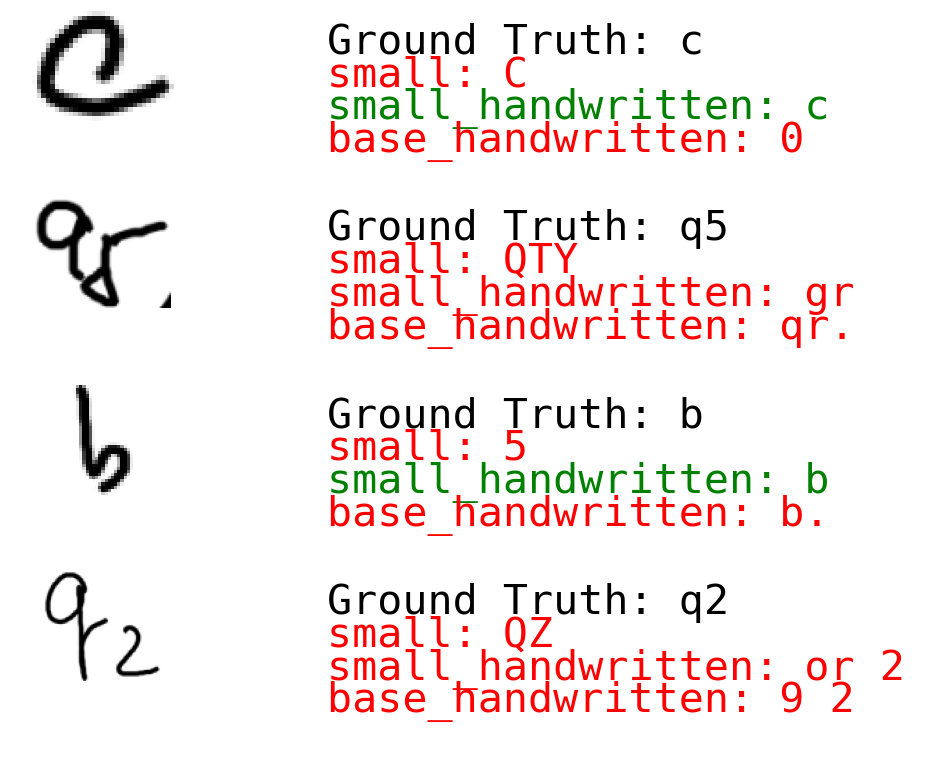
\includegraphics[width=\linewidth]{text_digitization_results_2.png}
\caption{Some results in which the \textit{trocr-base-handwritten} fails.}
\label{fig:text_digitization_results_2}
\end{figure}

\section{Discussion}
TODO

\section{Conclusion and Future Work}
TODO

\bibliographystyle{IEEEtran}
\bibliography{references}

\end{document}
